\chapter{Theoretical background}
\label{cap:fundamentacao}
\section{Quantum states}
A pure qubit is a normalized vector in a two-dimensional Hilbert space:
\begin{equation}\label{eq:qubit}
\lvert\psi\rangle=\alpha\lvert0\rangle+\beta\lvert1\rangle,\quad |\alpha|^{2}+|\beta|^{2}=1.
\end{equation}
The von Neumann entropy of a density operator is
\begin{equation}\label{eq:entropia}
S(\rho)=-\operatorname{Tr}(\rho\log_{2}\rho).
\end{equation}
Quantum coding was investigated by \textcite{schumacher1995}.

\section{Schematic representation}
Figure~\ref{fig:fluxo} represents a simplified preparation and processing sequence.
\begin{figure}[htbp]
\centering
\caption{State preparation and processing.}\label{fig:fluxo}
\vspace{.35cm}
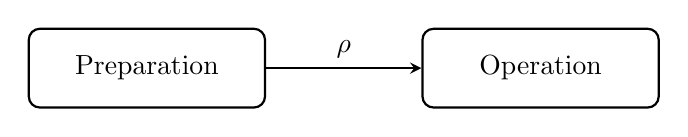
\begin{tikzpicture}[>=stealth,thick]
\node[draw,rounded corners,minimum width=3cm,minimum height=1cm] (a) at (0,0) {Preparation};
\node[draw,rounded corners,minimum width=3cm,minimum height=1cm] (b) at (5,0) {Operation};
\draw[->] (a) -- node[above] {$\rho$} (b);
\end{tikzpicture}
\par\medskip
\begin{minipage}{.55\textwidth}
\raggedright\footnotesize Source: prepared for this example.
\end{minipage}
\end{figure}
